% ----------------------------------------------------------------------
\section{Determinants of \texorpdfstring{$2\times 2$}{2x2}- and \texorpdfstring{$3\times 3$}{3x3}-matrices}

Let $A$ be an $n\times n$-matrix. The \textbf{determinant}%
\index{determinant} of $A$, denoted by $\det(A)$, is a very important
number which we will explore throughout this chapter.

The determinant of a$2\times 2$-matrix is given by the following
formula.

\begin{definition}{Determinant of a $2\times 2$-matrix}{two-by-two-determinant}
  Let $A=\begin{mymatrix}{rr}
    a & b \\
    c & d
  \end{mymatrix}$. Then
  \begin{equation*}
    \det(A) = ad-bc.
  \end{equation*}
\end{definition}

\begin{example}{A $2\times 2$ determinant}{two-by-two-determinant}
  Find $\det(A)$ for the matrix
  $A =  \begin{mymatrix}{rr}
    2 & 4 \\
    -1 & 6
  \end{mymatrix}$.
\end{example}

\begin{solution}
  We have $\det(A) = 2\cdot 6 - (-1)\cdot 4 = 12 + 4 = 16$.
\end{solution}

The determinant is also often denoted by enclosing the matrix with two
vertical lines. Thus
\begin{equation*}
  \det \begin{mymatrix}{cc}
    a & b \\
    c & d
  \end{mymatrix} =\begin{absmatrix}{cc}
    a & b \\
    c & d
  \end{absmatrix}
  = ad - bc.
\end{equation*}

\begin{definition}{Determinant of a $3\times 3$-matrix}{3-by-3-determinant}
  Let $A=\begin{mymatrix}{ccc}
    a_{11} & a_{12} & a_{13} \\
    a_{21} & a_{22} & a_{23} \\
    a_{31} & a_{32} & a_{33} \\
  \end{mymatrix}$. Then
  \begin{equation*}
    \det(A)
    = a_{11}a_{22}a_{33}
    + a_{12}a_{23}a_{31}
    + a_{13}a_{21}a_{32}
    - a_{31}a_{22}a_{13}
    - a_{32}a_{23}a_{11}
    - a_{33}a_{21}a_{12}.
  \end{equation*}
\end{definition}

The following picture helps in memorizing the formula:
\begin{equation*}
  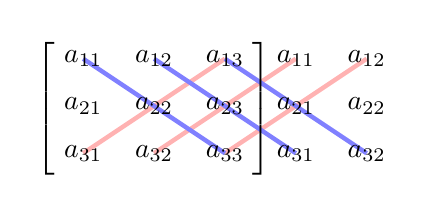
\begin{tikzpicture}[yscale=0.6,xscale=0.9]
    \draw[ultra thick,red!30] (1,-3) -- (3,-1);
    \draw[ultra thick,red!30] (2,-3) -- (4,-1);
    \draw[ultra thick,red!30] (3,-3) -- (5,-1);
    \draw[ultra thick,blue!50] (1,-1) -- (3,-3);
    \draw[ultra thick,blue!50] (2,-1) -- (4,-3);
    \draw[ultra thick,blue!50] (3,-1) -- (5,-3);
    \foreach\i in {1,2,3} {
      \foreach\j in {1,2,3} {
        \path (\j,-\i) node {$a_{\i\j}$};
      }
    }
    \foreach\i in {1,2,3} {
      \foreach\j in {1,2} {
        \path (\j,-\i) + (3,0) node {$a_{\i\j}$};
      }
    }
    \draw(0.5,-2) node {$\left[\rule{0mm}{1.0cm}\right.$};
    \draw(3.5,-2) node {$\left.\rule{0mm}{1.0cm}\right]$};
  \end{tikzpicture}
\end{equation*}

\begin{example}{A $3\times 3$ determinant}{3-by-3-determinant}
  Find $\det(A)$, where
  \begin{equation*}
    A = \begin{mymatrix}{rrr}
      0 & 1 & 2 \\
      3 & 1 & 0 \\
      1 & 1 & -1 \\
    \end{mymatrix}.
  \end{equation*}
\end{example}

\begin{solution}
  We have
  \begin{equation*}
    \det(A) ~=~
    \begin{absmatrix}{rrr}
      0 & 1 & 2 \\
      3 & 1 & 0 \\
      1 & 1 & -1 \\
    \end{absmatrix}
    ~=~
    0\cdot 1\cdot (-1)
    + 1\cdot 0 \cdot 1
    + 2 \cdot 3 \cdot 1
    - 1\cdot 1\cdot 2
    - 1\cdot 0\cdot 0
    - (-1)\cdot 3\cdot 1
    ~=~ 7.
  \end{equation*}
\end{solution}

% ----------------------------------------------------------------------
\section{Minors and cofactors}

Determinants of larger matrices can be computed in terms of the
determinants of smaller matrices. We begin with the following
definition.

\begin{definition}{The $\ijth$ minor of a matrix}{ijth-minor}
  Let $A$ be an $n\times n$-matrix. The $\ijth$ \textbf{minor}%
  \index{matrix!minor}%
  \index{determinant!minor}%
  \index{minor!of a matrix} of $A$, denoted by $\minor{A}{ij}$, is the
  determinant of the $(n-1)\times(n-1)$-matrix that is obtained by
  deleting the $i\th$ row and the $j\th$ column of $A$.
\end{definition}

Hence, there is a minor associated with each entry of $A$. The
following example illustrates this definition.

\begin{example}{Finding minors of a matrix}{finding-minors}
  Let
  \begin{equation*}
    A = \begin{mymatrix}{rrr}
      1 & 2 & 3 \\
      4 & 3 & 2 \\
      3 & 2 & 1
    \end{mymatrix}
  \end{equation*}
  Find the minors $\minor{A}{12}$ and $\minor{A}{33}$.
\end{example}

\begin{solution}
  First we will find $\minor{A}{12}$. By definition, this is the
  determinant of the $2\times 2$-matrix that results when we delete
  the first row and the second column of $A$. This minor is given by
  \begin{equation*}
    \minor{A}{12}
    ~=~
    \begin{absmatrix}{ccc}
      \strikeh{3.2em}{1} & \strikev{3.2em}{2} & 3 \\
      4 & 3 & 2 \\
      3 & 2 & 1 \\
    \end{absmatrix}
    ~=~
    \begin{absmatrix}{rr}
      4 & 2 \\
      3 & 1
    \end{absmatrix}
    ~=~ 4\cdot 1 - 3\cdot 2
    ~=~ -2. 
  \end{equation*}
  Similarly, $\minor{A}{33}$ is the determinant of the
  $2\times 2$-matrix that is obtained by deleting the third row and
  the third column of $A$. This minor is therefore
  \begin{equation*}
    \minor{A}{23}
    ~=~
    \begin{absmatrix}{ccc}
      1 & 2 & \strikev{3.2em}{3} \\
      4 & 3 & 2 \\
      \strikeh{3.2em}{3} & 2 & 1 \\
    \end{absmatrix}
    ~=~
    \begin{absmatrix}{rr}
      1 & 2 \\
      4 & 3
    \end{absmatrix}
    ~=~ -5.
  \end{equation*}
\end{solution}

We now define the $\ijth$ cofactor of a matrix $A$, which is either
plus or minus the $\ijth$ minor. 

\begin{definition}{The $\ijth$ cofactor of a matrix}{ijth-cofactor}
  Suppose $A$ is an $n\times n$-matrix. The $\ijth$ \textbf{cofactor}%
  \index{matrix!cofactor}%
  \index{determinant!cofactor}%
  \index{cofactor!of a matrix}, denoted by $\cof{A}{ij}$, is
  defined to be
  \begin{equation*}
    \cof{A}{ij} = (-1)^{i+j} \minor{A}{ij}
  \end{equation*}
\end{definition}

In other words, the $\ijth$ cofactor is equal to the corresponding
minor if $i+j$ is even, and the negative of the minor if $i+j$ is
odd. For remembering the signs, the following picture is sometimes
helpful:
\begin{equation*}
  \begin{mymatrix}{cccc}
    + & - & + & - \\
    - & + & - & + \\
    + & - & + & - \\
    - & + & - & + \\
  \end{mymatrix}.
\end{equation*}

\begin{example}{Finding cofactors of a matrix}{finding-cofactors}
  Consider the matrix
  \begin{equation*}
    A=\begin{mymatrix}{rrr}
      1 & 2 & 3 \\
      4 & 3 & 2 \\
      3 & 2 & 1
    \end{mymatrix}
  \end{equation*}
  Find the cofactors $\cof{A}{12}$ and $\cof{A}{33}$.
\end{example}

\begin{solution}
  We have already computed the corresponding minors in
  Example~\ref{exa:finding-minors}. For the cofactors, we have:
  \begin{eqnarray*}
    \cof{A}{12} &=& (-1)^{1+2}\minor{A}{12} ~=~ -\minor{A}{12} ~=~ -(-2) ~=~ 2,\\
    \cof{A}{33} &=& (-1)^{3+3}\minor{A}{33} ~=~ +\minor{A}{33} ~=~ +(-5) ~=~ -5.\\
  \end{eqnarray*}
  Note that $1+2$ is odd, so $\cof{A}{12}=-\minor{A}{12}$. On the
  other hand, $3+3$ is even, so $\cof{A}{33}=\minor{A}{33}$.
\end{solution}

You may wish to find the remaining cofactors of the above
matrix. Remember that there is a cofactor for every entry in the
matrix.

We have now established the tools we need to find the determinant of
an $n\times n$-matrix.

\begin{definition}{The determinant of an $n\times n$-matrix}{n-by-n-determinant}
  Let $A$ be an $n\times n$-matrix. Then $\det(A)$ is calculated by
  picking a row (or column) and taking the product of each entry in
  that row (column) with its cofactor and adding these products
  together. This process is known as \textbf{expanding along the
    $i\th$ row (or column)}%
  \index{determinant!expanding along row or column}.
  \bigskip
  
  In formulas, the process of expanding along the $i\th$ row is given
  as follows:
  \begin{equation*}
    \det(A) =
    a_{i1}\cof{A}{i1} + a_{i2}\cof{A}{i2} + \ldots + a_{in}\cof{A}{in}.
  \end{equation*}
  Similarly, the process of expanding along the $j\th$ column is:
  \begin{equation*}
    \det(A) =
    a_{1j}\cof{A}{1j} + a_{2j}\cof{A}{2j} + \ldots + a_{nj}\cof{A}{nj}.
  \end{equation*}
  
\end{definition}

When calculating the determinant, you can choose to expand any row or
any column. Regardless of which row or column you expand, you will
always get the same number, which is the determinant of the matrix
$A$.  This method of evaluating a determinant by expanding along a row
or a column is also called \textbf{cofactor expansion}%
\index{determinant!cofactor expansion}%
\index{cofactor expansion} or \textbf{Laplace expansion}%
\index{determinant!Laplace expansion}%
\index{Laplace expansion}.

\begin{example}{Finding a determinant by cofactor expansion}{determinant-three-by-three}
  Find $\det(A)$ using the method of cofactor expansion, where
  \begin{equation*}
    A = \begin{mymatrix}{rrr}
      1 & 2 & 3 \\
      4 & 3 & 2 \\
      3 & 2 & 1
    \end{mymatrix}.
  \end{equation*}
\end{example}

\begin{solution}
  First, we will calculate $\det(A)$ by expanding along the first
  column.  Using Definition~\ref{def:n-by-n-determinant}, the
  determinant is
  \begin{eqnarray*}
    \det(A)
    &=& a_{11}\cof{A}{11} + a_{21}\cof{A}{21} + a_{31}\cof{A}{31} \\
    &=& a_{11}\minor{A}{11} - a_{21}\minor{A}{21} + a_{31}\minor{A}{31} \\\\[-2ex]
    &=&
        1 \begin{absmatrix}{rr}
          3 & 2 \\
          2 & 1 \\
        \end{absmatrix}
        -4 \begin{absmatrix}{rr}
          2 & 3 \\
          2 & 1 \\
        \end{absmatrix}
        +3 \begin{absmatrix}{rr}
          2 & 3 \\
          3 & 2
        \end{absmatrix} \\\\[-1ex]
    &=& 1 (-1) - 4 (-4) + 3 (-5) \\
    &=& 0.
  \end{eqnarray*}
  As mentioned in Definition~\ref{def:n-by-n-determinant}, we
  can choose to expand along any row or column. Let's try now by
  expanding along the second row. The calculation is as follows.
  \begin{equation*}
    \det(A)
    ~=~ -4 \begin{absmatrix}{rr}
      2 & 3 \\
      2 & 1
    \end{absmatrix}
    +3 \begin{absmatrix}{rr}
      1 & 3 \\
      3 & 1
    \end{absmatrix}
    -2 \begin{absmatrix}{rr}
      1 & 2 \\
      3 & 2
    \end{absmatrix}
    ~=~ -4(-4) + 3(-8) - 2(-4)
    ~=~ 0.
  \end{equation*}
  You can see that for both methods, we obtained $\det(A) = 0$.
\end{solution}

You should try to compute the above determinant by expanding along
other rows and columns. This is a good way to check your work, because
you should come up with the same number each time!

\begin{theorem}{The determinant is well defined}{well-defined-determinant}
  Expanding the $n\times n$-matrix along any row or column always
  gives the same answer, which is the determinant.
\end{theorem}

\begin{example}{Determinant of a four by four matrix}{four-by-four-determinant}
  Calculate
  $\begin{absmatrix}{rrrr}
    1 & 2 & 3 & 0 \\
    2 & 4 & 2 & 3 \\
    0 & 3 & 0 & 5 \\
    3 & 0 & 3 & 2
  \end{absmatrix}$.
\end{example}

\begin{solution}
  Using the cofactor method, we can expand this determinant along any
  row or column. But notice that the third row contains two zeros.
  This makes the cofactor expansion particularly convenient. So let us
  expand along the third row. We have:
  \begin{equation*}
    \begin{absmatrix}{rrrr}
      1 & 2 & 3 & 0 \\
      2 & 4 & 2 & 3 \\
      0 & 3 & 0 & 5 \\
      3 & 0 & 3 & 2
    \end{absmatrix}
    =
    0 \begin{absmatrix}{rrrr}
      2 & 3 & 0 \\
      4 & 2 & 3 \\
      0 & 3 & 2
    \end{absmatrix}
    -3 \begin{absmatrix}{rrrr}
      1 & 3 & 0 \\
      2 & 2 & 3 \\
      3 & 3 & 2
    \end{absmatrix}
    +0 \begin{absmatrix}{rrrr}
      1 & 2 & 0 \\
      2 & 4 & 3 \\
      3 & 0 & 2
    \end{absmatrix}
    -5 \begin{absmatrix}{rrrr}
      1 & 2 & 3 \\
      2 & 4 & 2 \\
      3 & 0 & 3
    \end{absmatrix}.
  \end{equation*}
  Note that we only need to compute two of the $3\times 3$
  determinants, since the remaining two are multiplied by $0$. We can
  compute each $3\times 3$ determinant using the method of
  Definition~\ref{def:3-by-3-determinant}. We find:
  \begin{equation*}
    \begin{absmatrix}{rrrr}
      1 & 2 & 3 & 0 \\
      2 & 4 & 2 & 3 \\
      0 & 3 & 0 & 5 \\
      3 & 0 & 3 & 2
    \end{absmatrix}
    =
    -3 \begin{absmatrix}{rrrr}
      1 & 3 & 0 \\
      2 & 2 & 3 \\
      3 & 3 & 2
    \end{absmatrix}
    -5 \begin{absmatrix}{rrrr}
      1 & 2 & 3 \\
      2 & 4 & 2 \\
      3 & 0 & 3
    \end{absmatrix}
    = -3 \cdot 10 - 5\cdot (-24)
    = 90.
  \end{equation*}
\end{solution}

We remark that the cofactor expansion is mainly useful for calculating
determinants of small matrices, or matrices containing many
zeros. Indeed, imagine calculating the determinant of a
$10\times 10$-matrix by the cofactor method. This requires calculating
the determinants of ten $9\times 9$-matrices, each of which requires
calculating the determinants of nine $8\times 8$-matrices, each of
which requires calculating the determinants of eight
$7\times 7$-matrices, and so on. Calculating the determinant of a
$10\times 10$-matrix by the cofactor method would therefore require
$10\cdot 9\cdot 8\cdot \ldots \cdot 2\cdot 1 = 3628800$ steps! 

In the next few sections, we will explore some important properties
and characteristics of the determinant, including a much more
efficient method of calculating determinants of large matrices.
